\section{Historique}
%3
\begin{frame}
    \frametitle{L'évolution des cartes graphiques.}
\begin{block}{Années 1980 : contrôleurs video.}
  Ces circuits permettaient d'afficher sur un tube cathodique 
  des informations stockées en mémoire. Ils fournissaient des fonctionnalités de base, essentiellement orientées
  autour de la gestion de la mémoire vidéo et de la génération des signaux de synchronisation. 
  \begin{figure}[ht]
    \centering
    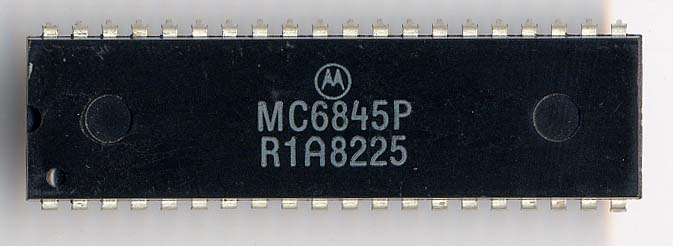
\includegraphics[scale=0.5]{Motorola_MC6845.jpg}
    \caption{Le contrôleur vidéo MC6845. \footnote{\tiny \url{https://commons.wikimedia.org/w/index.php?curid=976920}}}
    \label{fig:MC6845}
  \end{figure}
\end{block}
\end{frame}
%4
\begin{frame}
  \frametitle{L'évolution des cartes graphiques.}
\begin{block}{Contrôleurs graphiques}
  Apparus vers la fin des années 1980, ils apportent des fonctionnalités graphiques, telles le tracé de segment, 
  et gèrent une mémoire distincte de celle de l'unité centrale.
   \begin{figure}[htbp]
    \centering
    \hfill
   \begin{subfigure}{0.4\textwidth}
    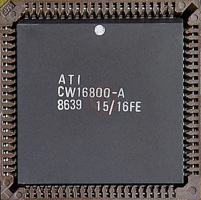
\includegraphics[scale=0.45]{ATI16800.jpg}
   \end{subfigure} 
   \hfill
   \begin{subfigure}{0.4\textwidth}
    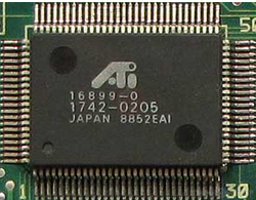
\includegraphics[scale=0.45]{ATI16899.jpg}
   \end{subfigure} 
   \hfill
    \caption{Contrôleurs graphiques.}
    \label{fig:graphic_controllers}
   \end{figure}
\end{block}
\end{frame}
%5
\begin{frame}
  \frametitle{L'évolution des cartes graphiques.}
\begin{block}{Les processeurs graphiques 3D.}
    Disponibles pour le grand public depuis le milieu des années 1990, ils incluent des fonctionalités
    d'affichage en trois dimensions. Parallèlement, des bibliothèques logicielles font leur apparition
    (OpenGL, Direct3D). L'affichage d'une scène est réalisé à travers un pipeline graphique: 
    transformation de sommets, projection, traçage.
    \begin{figure}[htbp]
        \centering
       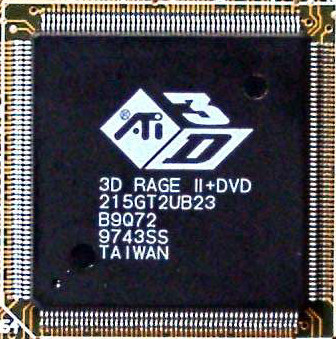
\includegraphics[scale=0.2]{3drage.jpg} 
        \caption{Contrôleur 3D ATI Rage.}
        \label{fig:ati_rage}
    \end{figure}
\end{block}
\end{frame}
%6
\begin{frame}
  \frametitle{L'évolution des cartes graphiques.}
\begin{block}{Les processeurs progammables.}
    En 2001, la société NVIDIA introduit sur le marché la gamme de processeurs graphiques
    GeForce 3 qui permettent de programmer les étapes du pipeline graphique. 
    \begin{figure}[htbp]
        \centering
       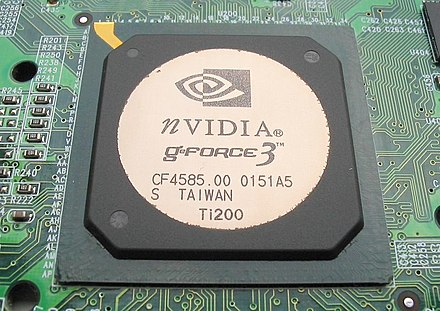
\includegraphics[scale=0.3]{Geforce3gpu.jpg} 
        \caption{Contrôleur 3D programmable.}
        \label{fig:geforce3}
    \end{figure}
\end{block}
%7
\end{frame}

\begin{frame}
  \frametitle{L'évolution des cartes graphiques.}
\begin{block}{Le calcul.}
    Fin 2006, NVIDIA lance la gamme GeForce 8 et l'environnement de développement CUDA qui
    permet d'exploiter la puissance de calcul des cartes graphiques pour des applications générales.
    Les performances théoriques sont impressionnantes, de l'ordre de celles obtenues avec un 
    superordinateur pour uen enveloppe énergétique comparable.

    \begin{figure}[htbp]
        \centering
       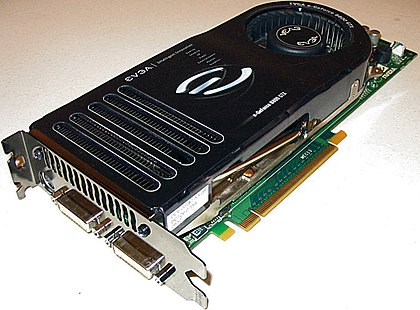
\includegraphics[scale=0.3]{geforce8800.jpg} 
        \caption{Carte graphique CUDA.}
        \label{fig:gforce8}
    \end{figure}
\end{block}
\end{frame}

\begin{frame}
  \frametitle{Synthèse de l'évolution des cartes NVIDIA}
{\footnotesize  
\hspace{-1cm}
            \begin{tabular}{p{3cm}p{1.5cm}p{3.5cm}p{1cm}p{1cm}p{1cm}}
            \rowcolor{lightgray}\textbf{Année} & \textbf{Carte} & \textbf{Architecture} & \textbf{Cœurs NVIDIA CUDA} & \textbf{RAM} & \textbf{Puissance} \\\hline
            1995 & NV1 & dizaines de micromètres (µm) & ?  & 2-4 Mo & 2 Watts \\
            ... & ... & ...  & ... & ... & ...\\
    
            2017 & GTX 1080 Ti & Volta 16 nm & 3584 & 11 Go & 257 watts \\
            2019 & GTX 2080 Ti & Turing 12 nm & 4352 & 11 Go & 290 Watts \\
            2020 & RTX 3090 & Ampere 8 nm & 10 496 & 24 Go & 350 Watts \\
            2022 & RTX 4090 & Ada Lovelace 4 nm & 18 000  & 24 Go & 450-600 Watts \\            
        \end{tabular}
\end{block}
\end{frame}
